% Chapter 1

\chapter{Introduction and Background} % Main chapter title

\label{Chapter1} % For referencing the chapter elsewhere, use \ref{Chapter1} or autoref{Chapter} or cref{}, or Cref{} 

%----------------------------------------------------------------------------------------

% Define some commands to keep the formatting separated from the content 
\newcommand{\keyword}[1]{\textbf{#1}}
\newcommand{\tabhead}[1]{\textbf{#1}}
\newcommand{\code}[1]{\texttt{#1}}
\newcommand{\file}[1]{\texttt{\bfseries#1}}
\newcommand{\option}[1]{\texttt{\itshape#1}}

%----------------------------------------------------------------------------------------


\section{Preliminaries}
\label{preliminaries}


\begin{figure*}
    \centering
    \begin{subfigure}[b]{0.25\textwidth}
        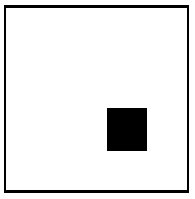
\includegraphics[width=\textwidth]{Figures/block-failure-pattern.pdf}
        \caption{Block}
        \label{fig:block-failure-pattern}
    \end{subfigure}
    \begin{subfigure}[b]{0.25\textwidth}
        
\includegraphics[width=\textwidth]{Figures/strip-failure-pattern.pdf}
        \caption{Strip}
        \label{fig:strip-failure-pattern}
    \end{subfigure}
    \begin{subfigure}[b]{0.25\textwidth}
        
\includegraphics[width=\textwidth]{Figures/point-failure-pattern.pdf}
        \caption{Point}
        \label{fig:point-failure-pattern}
    \end{subfigure}
    \caption{Failure Patterns}
    \label{Failure-Patterns}
\end{figure*}

Ed ut perspiciatis unde omnis~\cite{Duran1981} iste natus error sit voluptatem~\cite{Deza2009} accusantium doloremque laudantium, totam rem aperiam, eaque ipsa quae ab illo.

\begin{equation}
    NNS(q) = arg \min_{x \in X} \delta(q, x)
\end{equation}

inventore veritatis et qsed quia non numquam eius modi tempora incidunt ut labore et dolore magnam aliquam quaerat voluptatem\cite{hantler1976}. Ut enim ad minima veniam, quis nostrum exercitationem ullamulla pariatur.



\subsection{Previous works}
\label{Previous works}

% dummy text
\lipsum[1-3] % delete this line to add real abstract 
\begin{table*}[!t]
    \centering
    \caption{Discrepancy in Various Dimensions}
    \label{tbl_discrepancy}
    % \setlength{\extrarowheight}{2pt}
    \resizebox{\textwidth}{!}{%
    \begin{tabular}{ccccccccc}
        \hline
        \multirow{2}{*}{Test Cases} & \multirow{2}{*}{Method} & \multicolumn{7}{c}{Discrepancy} \\ \cline{3-9} 
         &  & 1-$d$ & 2-$d$ & 3-$d$ & 4-$d$ & 5-$d$ & 10-$d$ & 15-$d$ \\ \hline
        \multirow{3}{*}{100} & FSCS-ART & 0.0750 & 0.1393 & \textbf{0.2159} & 0.2697 & \textbf{0.3112} & 0.3135 & 0.3108 \\  
         & LimBal-KDFC & 0.0628 &\textbf{ 0.1295} & 0.2250 & 0.2856 & 0.3138 & 0.3070 & 0.2886 \\  
         & SWFC-ART & \textbf{0.0562} & 0.1359 & 0.2420 & \textbf{0.2652} & 0.3206 & \textbf{0.2942} & \textbf{0.2759} \\ \hline
        \multirow{3}{*}{1000} & FSCS-ART & 0.0181 & 0.0381 & 0.1036 & 0.1620 & 0.1899 & 0.2228 & 0.2090 \\  
         & LimBal-KDFC & \textbf{0.0163} & \textbf{0.0347} & 0.0961 & 0.1592 & 0.1884 & 0.2140 &\textbf{ 0.2055} \\  
         & SWFC-ART & 0.0168 & 0.0355 & \textbf{0.0930} & \textbf{0.1515} & \textbf{0.1739} & \textbf{0.2010} & 0.2106 \\ \hline
        \multirow{3}{*}{10,000} & FSCS-ART & \textbf{0.0084} & 0.0163 & 0.0574 & 0.1091 & 0.1534 & 0.1987 & 0.1889 \\  
         & LimBal-KDFC & 0.0085 & \textbf{0.0133} & 0.0560 & 0.1098 & \textbf{0.1385} & 0.1883 & 0.1859 \\  
         & SWFC-ART & 0.0089 & 0.0151 & \textbf{0.0525} & \textbf{0.1033} & 0.1388 & \textbf{0.1795} & \textbf{0.1623} \\ \hline
    \end{tabular}
    }
\end{table*}


